\documentclass{article}
\usepackage[utf8]{inputenc}
\usepackage{listings}
\usepackage{color}

\usepackage[left=2cm, right=2cm, top=2cm]{geometry}
\title{IO\_URING}
\author{Dinesh Reddy}
\date{April 2023}

\usepackage{graphicx}
\graphicspath{ {../report/} }
\usepackage[colorlinks=true, allcolors=blue]{hyperref}
\usepackage{listings}

\lstset{basicstyle=\footnotesize\ttfamily,breaklines=true}
\lstset{framextopmargin=5pt,frame=lrtb}

% REMEMBER TO SUBMIT YOUR CODE AND THE OUTPUT FILE FOR STRACE

\begin{document}
\maketitle
\section{Abstract}
With the slowing of Mores Law, hardware trends moved towards parallelism. This exposes the need for asynchronous
system calls. IO\_URING is a simple to use interface introduced in the recent Linux Kernels is being 
rapidly adapted for various IO -- network and block. We show the efficacy of IO\_URING in file-copy 
utilities by improving the performance by roughly an order of magnitude for copying medium and large files.

\section{IO\_URING}

Hardware is moving towards parallelism.

Linux aio is complicated.

IO\_URING uses shared memory between user and kernel space. Hence, we have advantages like "zero-copy", batching...

\section{Experimetal Setup}
\subsection{System Specifications}
I am using a Ubuntu 20 machine.

Though the selection of hardware doesn't clearly take advantage of performance benefits associated
with parallel hardware, we still get some advantage in terms of minimizing system calls and zero-copying.

We performaned every experiment 5 times. 

For the experiments involving IO\_URING benefits, we used 4K blocks. 

To make sure that block cache doesn't impact the performance, we mount a virtual disk and access 
the files from the virtual disk.

\noindent\begin{minipage}{.45\textwidth}
    \begin{lstlisting}[language=Bash, caption=Create a Virtual disk, basicstyle=\tiny]
sudo mkdir ./virtualdisk
sudo dd if=/dev/zero of=./virtualdisk/vdisk.img bs=1G count=10
sudo losetup /dev/loop40 ./virtualdisk/vdisk.img
sudo mkfs.ext4 /dev/loop40 
    \end{lstlisting}
    \end{minipage}\hfill
    \begin{minipage}{.45\textwidth}
    \begin{lstlisting}[language=Bash, caption=mount and unmount when using,frame=tlrb, basicstyle=\tiny]{Name}
sudo mount /dev/loop40 ./virtualdisk
sudo dd if=/dev/urandom of=./virtualdisk/largefile bs=1G count=1
# access the file
# ...
sudo umount virtualdisk
sudo losetup -d /dev/loop40
    \end{lstlisting}
    \end{minipage}


\subsection{Understanding metrics - Latency}
As shown in the pseudocode, we measure latency by the time it takes for the read to finish.

This would capture the time it takes 

\begin{lstlisting}[language=C, caption=Psudocode, basicstyle=\tiny]
int latency_main(int argc, char **argv) {
    fd = open("virtualdisk/largefile", O_RDONLY | O_DIRECT); // Open the file

    int block_num = opts.opt_random ? rand() % NUM_BLOCKS : 0;
    if(opts.opt_synchronous) ret = lseek(fd, block_num*BLOCK_SIZE, SEEK_SET);
    else io_uring_setup_and_init(block_num);

    gettimeofday(&submit_time, NULL); // after submitting all the request
    if(opts.opt_synchronous) ret = read(fd, read_buffer, BLOCK_SIZE);
    else{
        io_uring_submit(&ring); 
        ret = io_uring_wait_cqe(&ring, &cqe);
    }
    gettimeofday(&end_time, NULL); // End the timer
}

\end{lstlisting}

\begin{figure}
    \centering
    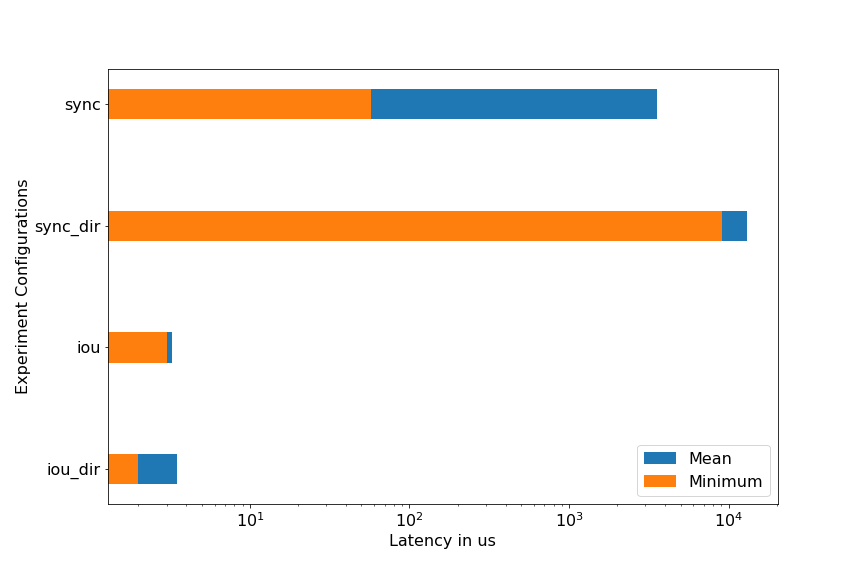
\includegraphics[scale = 0.25]{latency.png}
    \caption{4K block random read latency comparision.}
    \label{Figure1}
\end{figure}

\subsection{Understanding metrics - IOPS}

\begin{figure}
    \centering
    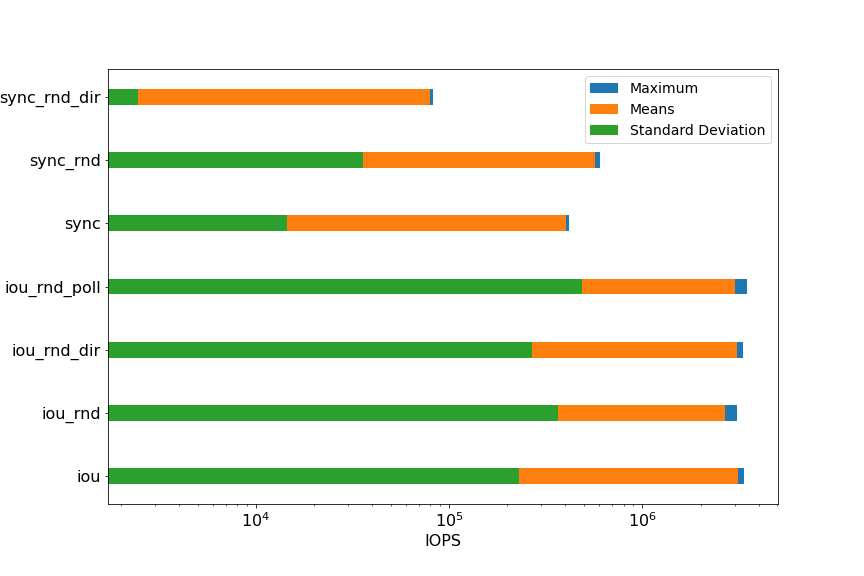
\includegraphics[scale = 0.25]{iops.png}
    \caption{4K block random read IOPS comparision.}
    \label{Figure2}
\end{figure}

\subsection{Types of experimets}

\section{Performance benefits of IO\_URING}
\subsection{Impact of Queue Depth}

\begin{figure}
    \centering
    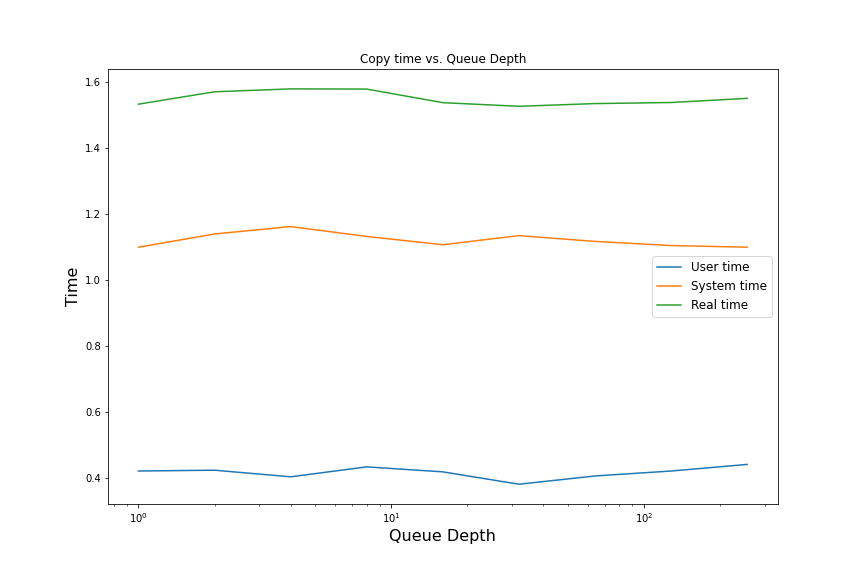
\includegraphics[scale = 0.25]{cp_qd.png}
    \caption{4K block random read latency comparision.}
    \label{Figure3}
\end{figure}

\begin{figure}
    \centering
    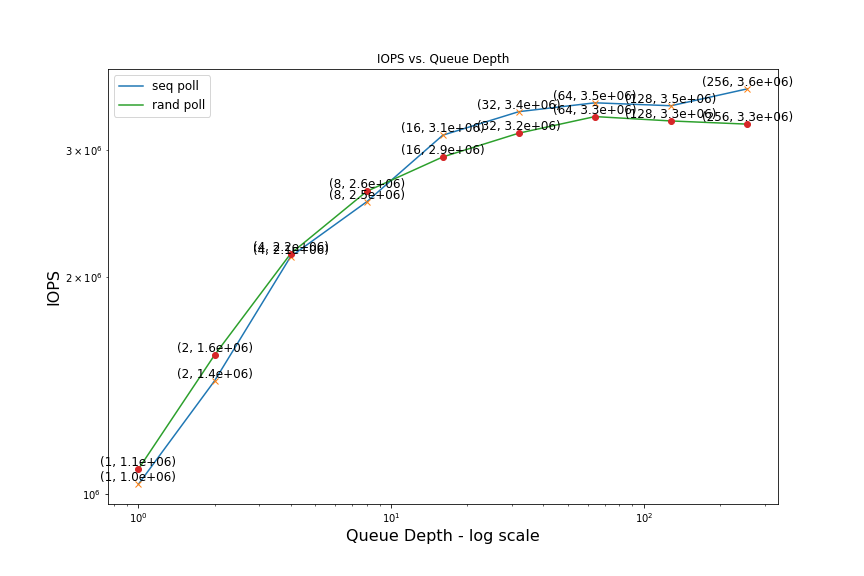
\includegraphics[scale = 0.25]{queue_depth.png}
    \caption{4K block random read latency comparision.}
    \label{Figure4}
\end{figure}


\subsection{Impact of Block Size}

\begin{figure}
    \centering
    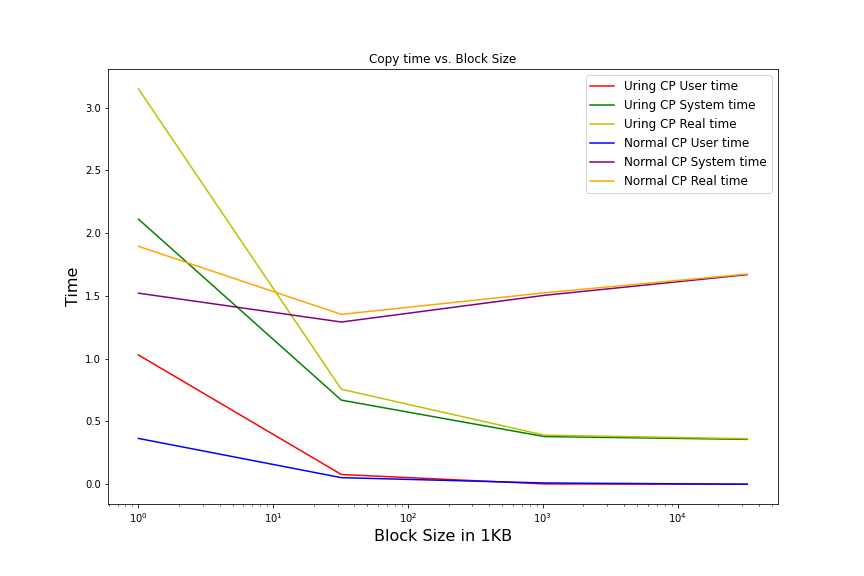
\includegraphics[scale = 0.25]{cp_bs.png}
    \caption{4K block random read latency comparision.}
    \label{Figure5}
\end{figure}

\section{Evaluation}
\subsection{cp vs uring\_cp}

\begin{figure}
    \centering
    
\includegraphics[scale = 0.5]{cp_perf_compare.png}
    \caption{4K block random read latency comparision.}
    \label{Figure6}
\end{figure}


\subsection{cp -r vs uring\_cp}

\begin{figure}
    \centering
    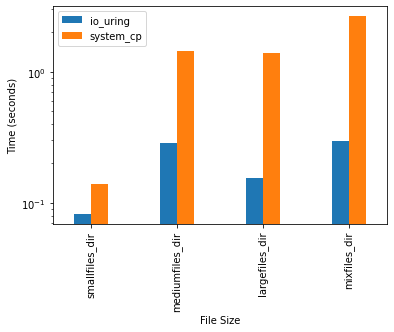
\includegraphics[scale = 0.5]{cp_perf_recursive_compare.png}
    \caption{4K block random read latency comparision.}
    \label{Figure7}
\end{figure}

\section{Conclusion}
IO\_URING is complicated to use. It is challenging not only to implement the functionality but also to harness 
the performance with correct configurations and settings.


\subsection{Referances}
Please find the code at my git repo \href{git@github.com:chintadinesh/adv\_os-project.git}{git@github.com:chintadinesh/adv\_os-project.git}.
\end{document}